% =============================================================================
%   Sistema Embarcado de Navegação Semi-Assistida para Cadeiras de Rodas
%   RELATÓRIO FINAL — Sistemas Operacionais Embarcados — UnB
%
%   Compilação:  pdflatex relatorio_final.tex && pdflatex relatorio_final.tex
%
%   Figuras usadas (todas presentes em docs/figs/):
%     Geradas do CSV real (odometria_20260709_151714.csv):
%       trajetoria.pdf  vel_rodas.pdf  vel_linear.pdf  vel_angular.pdf
%     Prints da GUI:
%       gui_tracao.jpeg  gui_lidar.jpeg  gui_odometria.png  gui_ajuste_pid.jpeg
%     Fotos:
%       cadeira_frente.jpeg  cadeira_lateral.jpeg  roda_motor.jpeg
%       terminais_alimentacao.jpeg  circuito_principal.jpeg
%   Presentes mas NÃO usadas: cadeira_geral, roda_e_encoder, gui_imu, gui_trajetoria
%   A Fig. do cone-vs-corredor é desenhada em TikZ (não precisa de arquivo).
% =============================================================================

\documentclass[conference]{IEEEtran}
\IEEEoverridecommandlockouts

\usepackage[utf8]{inputenc}
\usepackage[T1]{fontenc}
\usepackage[brazilian]{babel}
\usepackage{graphicx}
\usepackage{amsmath,amssymb}
\usepackage{cite}
\usepackage{url}
\usepackage{xcolor}
\usepackage{tikz}
\usepackage{listings}
\usepackage{siunitx}
\usetikzlibrary{shapes.geometric, arrows.meta, positioning, fit, backgrounds, calc}

\sisetup{output-decimal-marker={,}, per-mode=symbol, detect-all}
\DeclareSIUnit{\inch}{pol}
\DeclareSIUnit{\PPR}{PPR}

\graphicspath{{figs/}}
% Sem extensão nos \includegraphics: o LaTeX escolhe a que existir (.jpeg local, .jpg no Overleaf).
\DeclareGraphicsExtensions{.pdf,.png,.jpg,.jpeg}

\lstset{
  basicstyle=\ttfamily\footnotesize,
  breaklines=true,
  columns=fullflexible,
  keepspaces=true,
  frame=single,
  framesep=3pt,
  xleftmargin=2pt,
  xrightmargin=2pt
}

\begin{document}

\title{Sistema Embarcado de Navegação Semi-Assistida\\
para Cadeiras de Rodas Motorizadas:\\
Odometria de Encoders, Controle PID por Roda\\
e Supervisor de Segurança LiDAR}

\author{
\IEEEauthorblockN{Vítor Gonçalves de Andrade Silva — 261025182}
\IEEEauthorblockA{Faculdade de Ciências e Tecnologia em Engenharia\\
Engenharia Eletrônica\\
St. Leste Projeção A Gama Leste, Brasília -- DF, 72444-240\\
Email: 261025182@aluno.unb.br}
\and
\IEEEauthorblockN{Thiago Henrique Oliveira Souza — 180131672}
\IEEEauthorblockA{Faculdade de Ciências e Tecnologia em Engenharia\\
Engenharia Eletrônica\\
St. Leste Projeção A Gama Leste, Brasília -- DF, 72444-240\\
Email: 180131672@aluno.unb.br}
}

\maketitle

% =============================================================================
\begin{abstract}
Este relatório final consolida o sistema de direção semi-assistida para cadeiras
de rodas motorizadas desenvolvido ao longo dos Pontos de Controle 2 a 4. Sobre a
base estabelecida no PC4 --- protocolo serial com portão de segurança
(\texttt{drive\_cfg}) e condução assistida (\texttt{drive\_cmd}), ambos sob
\emph{watchdog} --- esta etapa entrega cinco avanços verificados
experimentalmente: (i)~\textbf{odometria de rodas} por encoders em quadratura
lidos pelo periférico PCNT do ESP32-S3, com calibração de aro e entre-eixos,
exportação de trajetória e integração ao ROS\,2 via \texttt{/wheel/odom};
(ii)~\textbf{malha de velocidade por roda} fechada no firmware, com o estado do
PID publicado em telemetria; (iii)~\textbf{interface gráfica de bancada}
reconstruída, com painéis de joystick, saída dos motores, LiDAR, IMU e odometria,
parada automática por zonas e ensaio de degrau; (iv)~\textbf{robustez
operacional}, incluindo religamento automático da ponte serial, nomeação estável
de portas e inicialização \emph{headless} por \texttt{systemd}; e
(v)~a~\textbf{correção de uma falha de segurança no supervisor}, cuja folga
frontal era medida por um cone angular ancorado no sensor --- construção válida
apenas se o LiDAR estivesse sobre o eixo do veículo. Estando ele
\SI{0.336}{\metre} fora do eixo, a metade direita da cadeira ficava cega
justamente nas curtas distâncias em que a parada precisa agir
(\SI{52}{\percent} de cobertura a \SI{0.60}{\metre}, \SI{23}{\percent} a
\SI{0.30}{\metre}); substituiu-se o cone por um teste de corredor no
\texttt{base\_link}, com a pose do sensor calibrada por três métodos
independentes e validada contra parede com erro de \SI{4}{\milli\metre}. Um
ensaio de condução no solo (\SI{58}{\second} de tráfego efetivo,
\SI{9.74}{\metre} de caminho) exercitou a odometria de encoders. O mesmo ensaio
expôs um defeito de medição de velocidade na camada de visualização ---
amostragem temporal por relógio de parede sob chegada em rajada da serial ---
aqui documentado e medido, com correção especificada mas ainda não aplicada.
Reporta-se ainda, com transparência, que o \emph{bloqueio direcional}
(parar o avanço preservando a ré) foi implementado mas contém um defeito de sinal
identificado em revisão de código e \textbf{não foi validado em hardware}.
\end{abstract}

% =============================================================================
\section{Introdução}

O projeto desenvolve um sistema de direção semi-assistida para cadeiras de rodas
motorizadas, voltado a usuários com deficiência motora severa, baixo controle de
tronco ou ausência de controle motor fino~\cite{fehr2000,branco2018}. Comandos
acidentais e espasmos no joystick podem produzir acelerações repentinas e
colisões; a literatura clínica aponta que parcela expressiva dos pacientes é
considerada inapta ao uso de cadeiras motorizadas justamente pela inadequação das
interfaces de controle~\cite{fehr2000}. A proposta converte a cadeira em um
veículo semi-autônomo sob modelo mestre--escravo: a Raspberry Pi~5, com
Ubuntu~24.04 e ROS\,2 Jazzy~\cite{ros2docs}, executa percepção e assistência de
alto nível, enquanto o ESP32-S3 mantém o laço de tempo real do joystick, dos
encoders e dos motores~\cite{ogata2010}.

O PC4 entregou o supervisor de segurança e o protocolo assistido, mas deixou três
lacunas explícitas: a telemetria de rodas não era usada para odometria fechada, o
desvio autônomo não fora exercitado com motor, e a parada por teto de \emph{duty}
inibia também a ré nas proximidades do obstáculo. Este relatório final ataca
essas lacunas e documenta o que foi --- e o que \emph{não} foi --- validado.
Exercitar o desvio com motor, em particular, revelou que o próprio supervisor
herdado do PC4 continha uma falha de segurança latente: sua noção de ``frente''
pressupunha um sensor centrado. O defeito, sua causa geométrica e a correção são
o objeto da Seção~\ref{sec:corredor}.

Contribuições desta etapa:

\begin{enumerate}
\item \textbf{Odometria de rodas por encoders}: leitura em quadratura 4$\times$
(\num{8000} contagens por volta) pelo PCNT, integração de pose por arco médio,
calibração ao vivo de aro e entre-eixos, exportação de trajetória em CSV e
publicação em \texttt{/wheel/odom}.

\item \textbf{Controle PID de velocidade por roda} no firmware, com
\emph{setpoints} enviados pelo host (\texttt{wheel\_speed\_cmd}) e estado do
controlador devolvido em telemetria (\texttt{/wheel/pid\_state}).

\item \textbf{Interface de bancada instrumentada}: painéis de joystick (com
inversão de eixos configurável), saída dos motores por GPIO, LiDAR com parada
automática por zonas, IMU e odometria com trajetória e velocidades; ensaio de
degrau; exportação de CSV.

\item \textbf{Robustez operacional}: religamento automático da ponte serial,
\emph{symlinks} \texttt{udev} estáveis, inicialização \emph{headless} via
\texttt{systemd} e diagnóstico de contenção de porta serial.

\item \textbf{Correção de uma falha de segurança geométrica}: substituição do
cone angular do supervisor por um teste de corredor no \texttt{base\_link}, com
calibração medida da pose do LiDAR e validação contra referência física
(Seção~\ref{sec:corredor}). Corrigiu-se também uma inconsistência dimensional no
desvio, em que um \emph{offset} de rumo era somado como velocidade angular.

\item \textbf{Achados negativos reportados}: um defeito de medição de velocidade
na GUI e um defeito de sinal no bloqueio direcional do firmware, ambos
caracterizados quantitativamente e não mascarados.
\end{enumerate}

% =============================================================================
\section{Plataforma}

A Fig.~\ref{fig:cadeira} mostra a base mecânica --- uma cadeira Ortobras AVD
convertida --- e a Fig.~\ref{fig:eletronica} a eletrônica embarcada. Cada roda
traseira recebe um motor DC de \SI{24}{\volt} acoplado ao aro e um encoder
incremental E6B2-CWZ1X (\num{2000}\,PPR) solidário ao eixo; as pontes BTS7960
recebem PWM complementar do ESP32-S3. A Fig.~\ref{fig:circuito} detalha o
circuito de controle e o condicionamento dos canais de encoder.

\begin{figure}[!t]
\centering
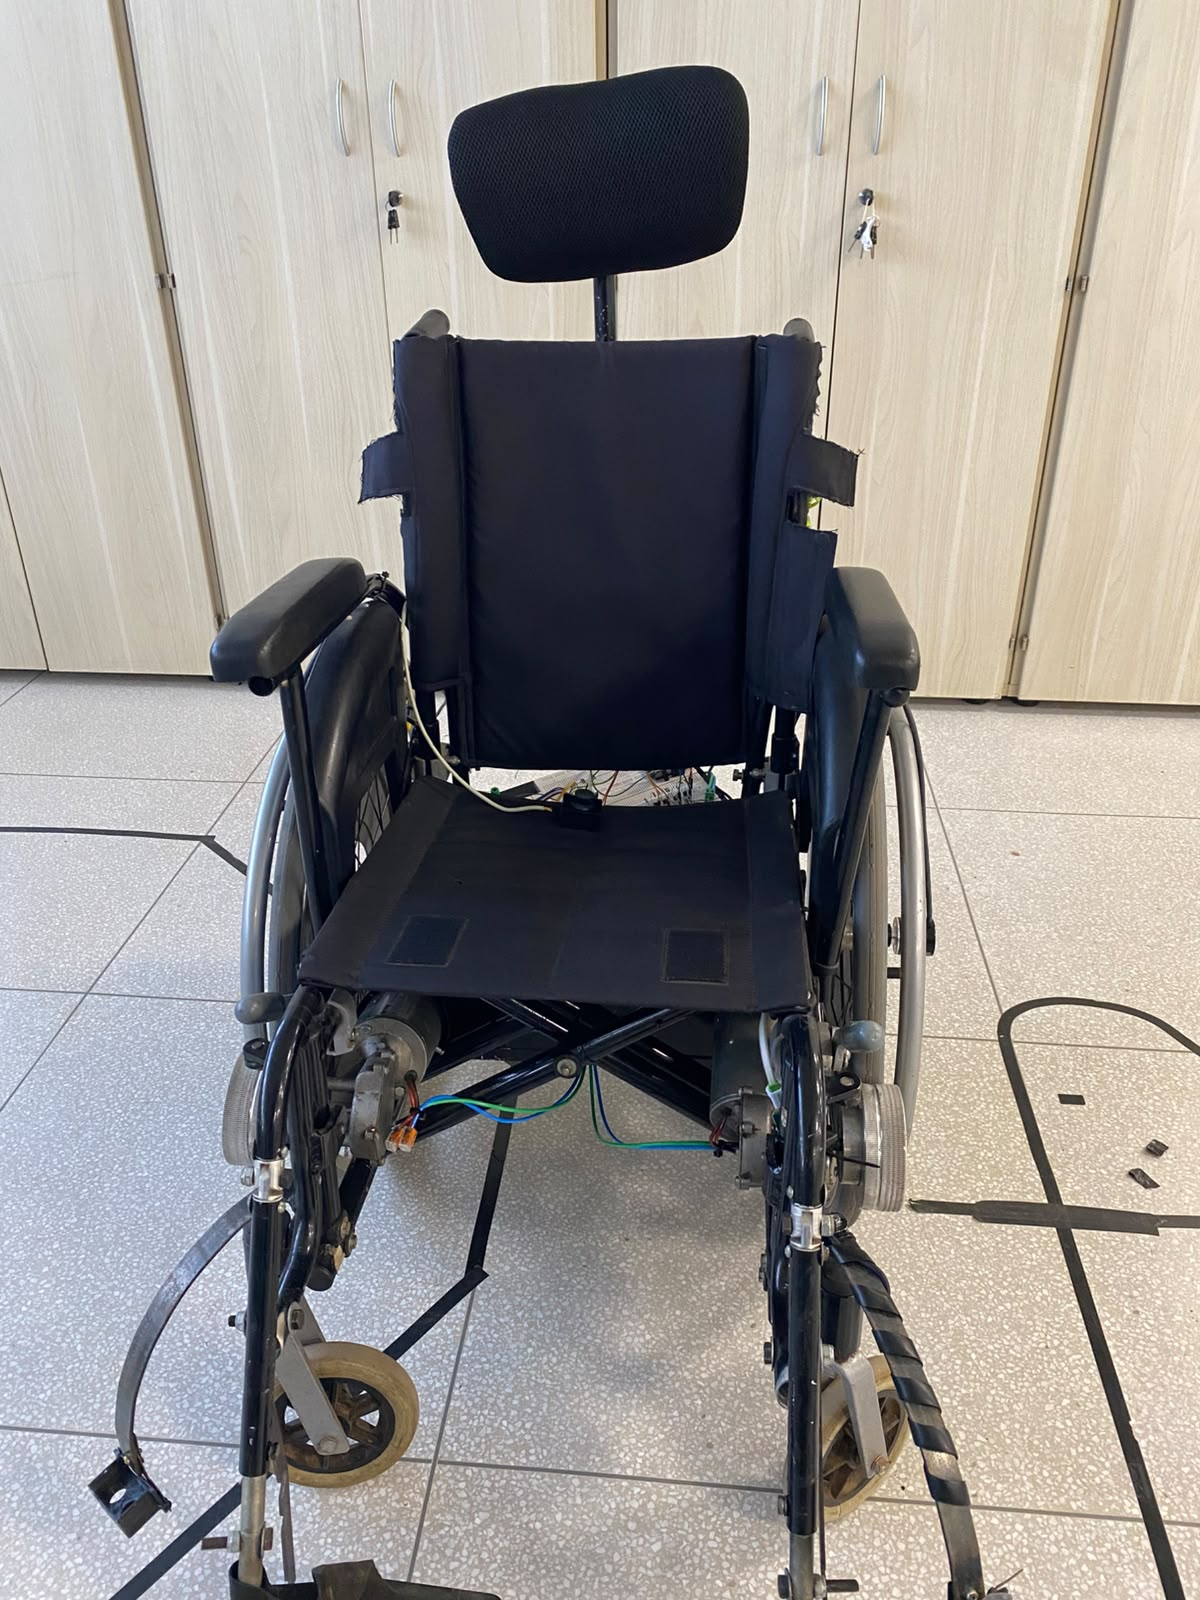
\includegraphics[width=0.46\columnwidth]{cadeira_frente}\hfill
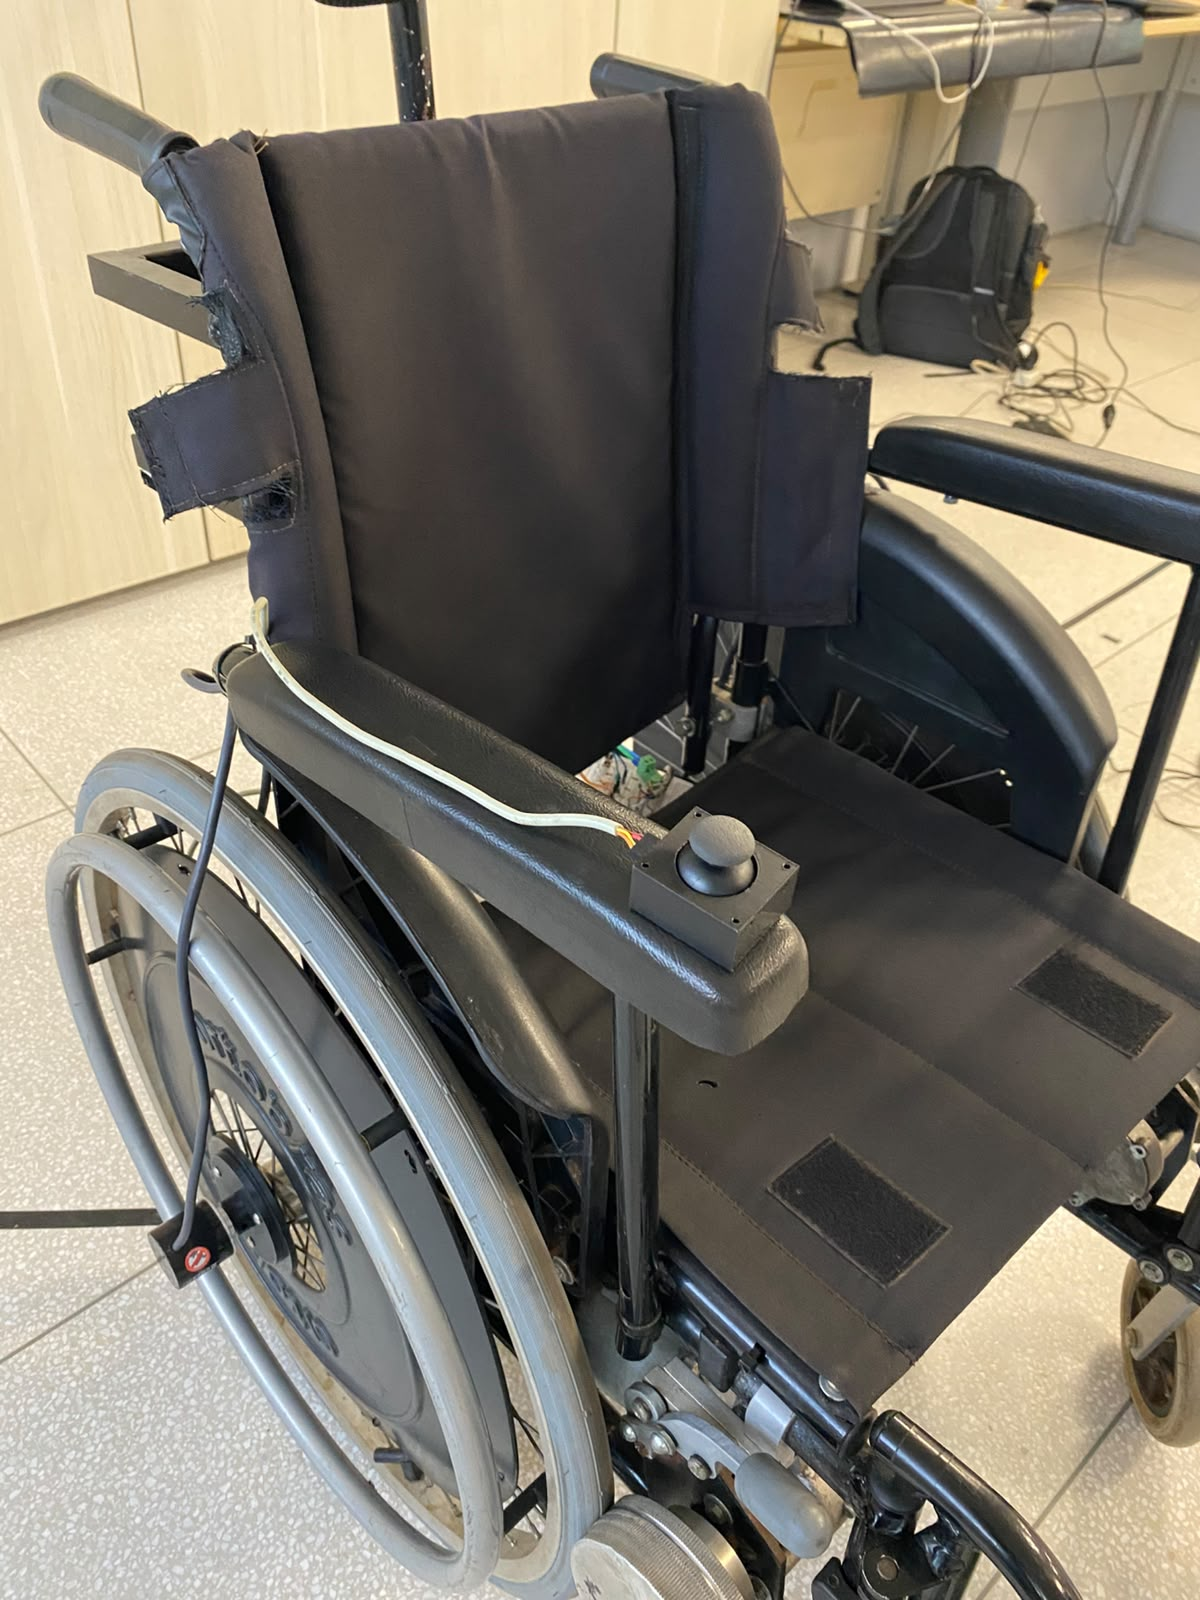
\includegraphics[width=0.46\columnwidth]{cadeira_lateral}
\caption{Base mecânica instrumentada. À esquerda, vista frontal com os dois
motores DC acoplados às rodas traseiras e a eletrônica sob o assento. À direita,
vista lateral com o joystick analógico montado no apoio de braço, mantendo a
ergonomia original da cadeira.}
\label{fig:cadeira}
\end{figure}

\begin{figure}[!t]
\centering
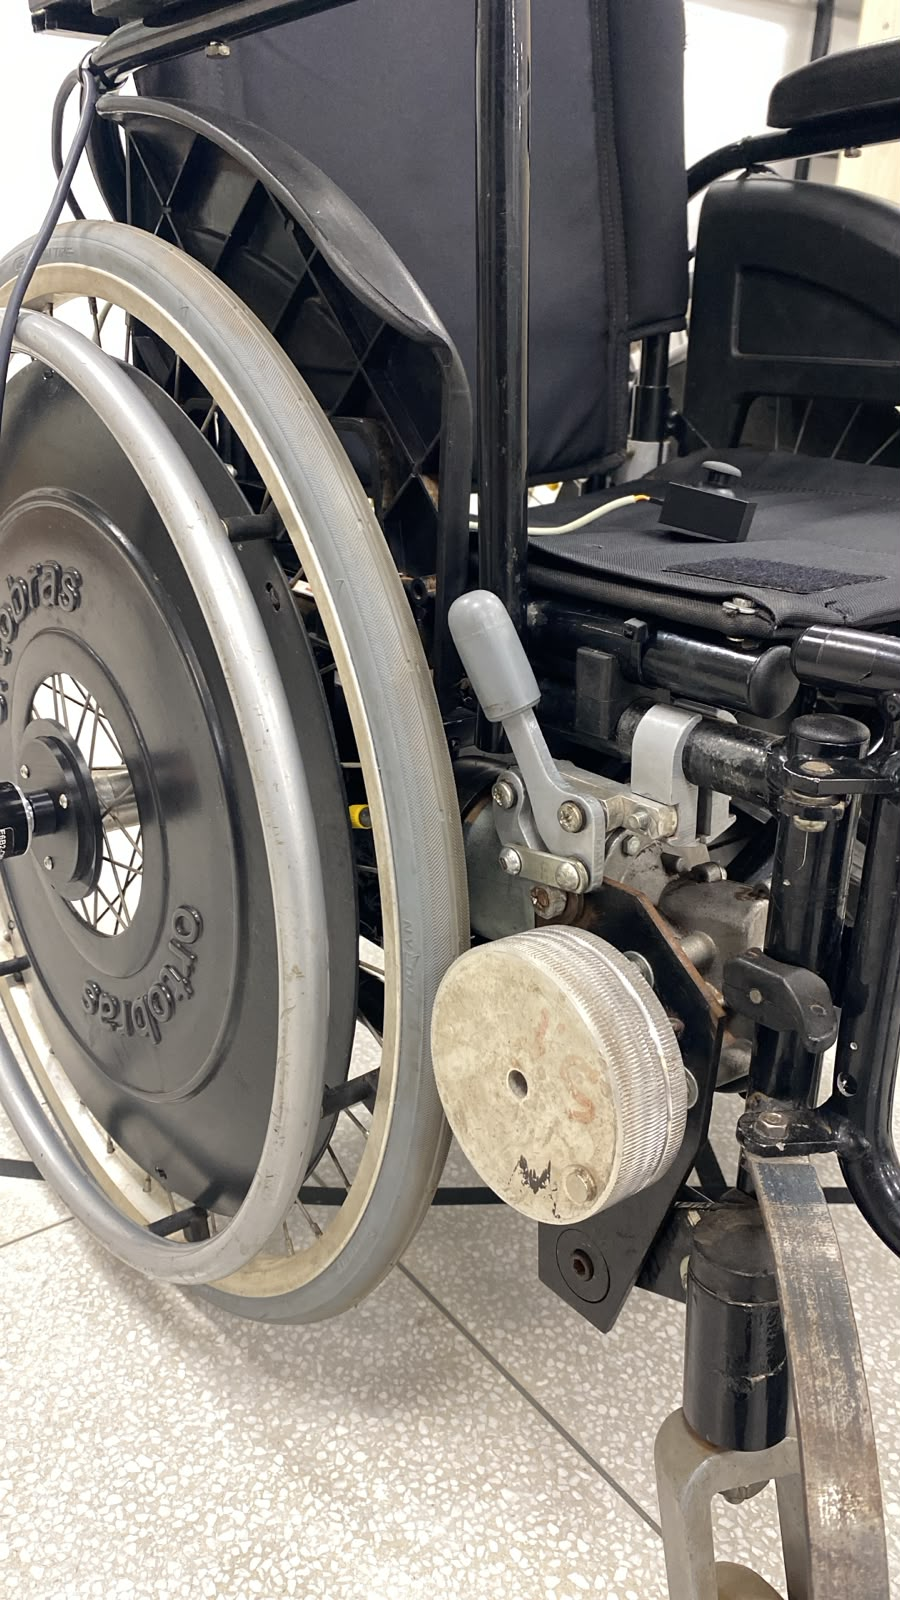
\includegraphics[width=0.48\columnwidth]{roda_motor}\hfill
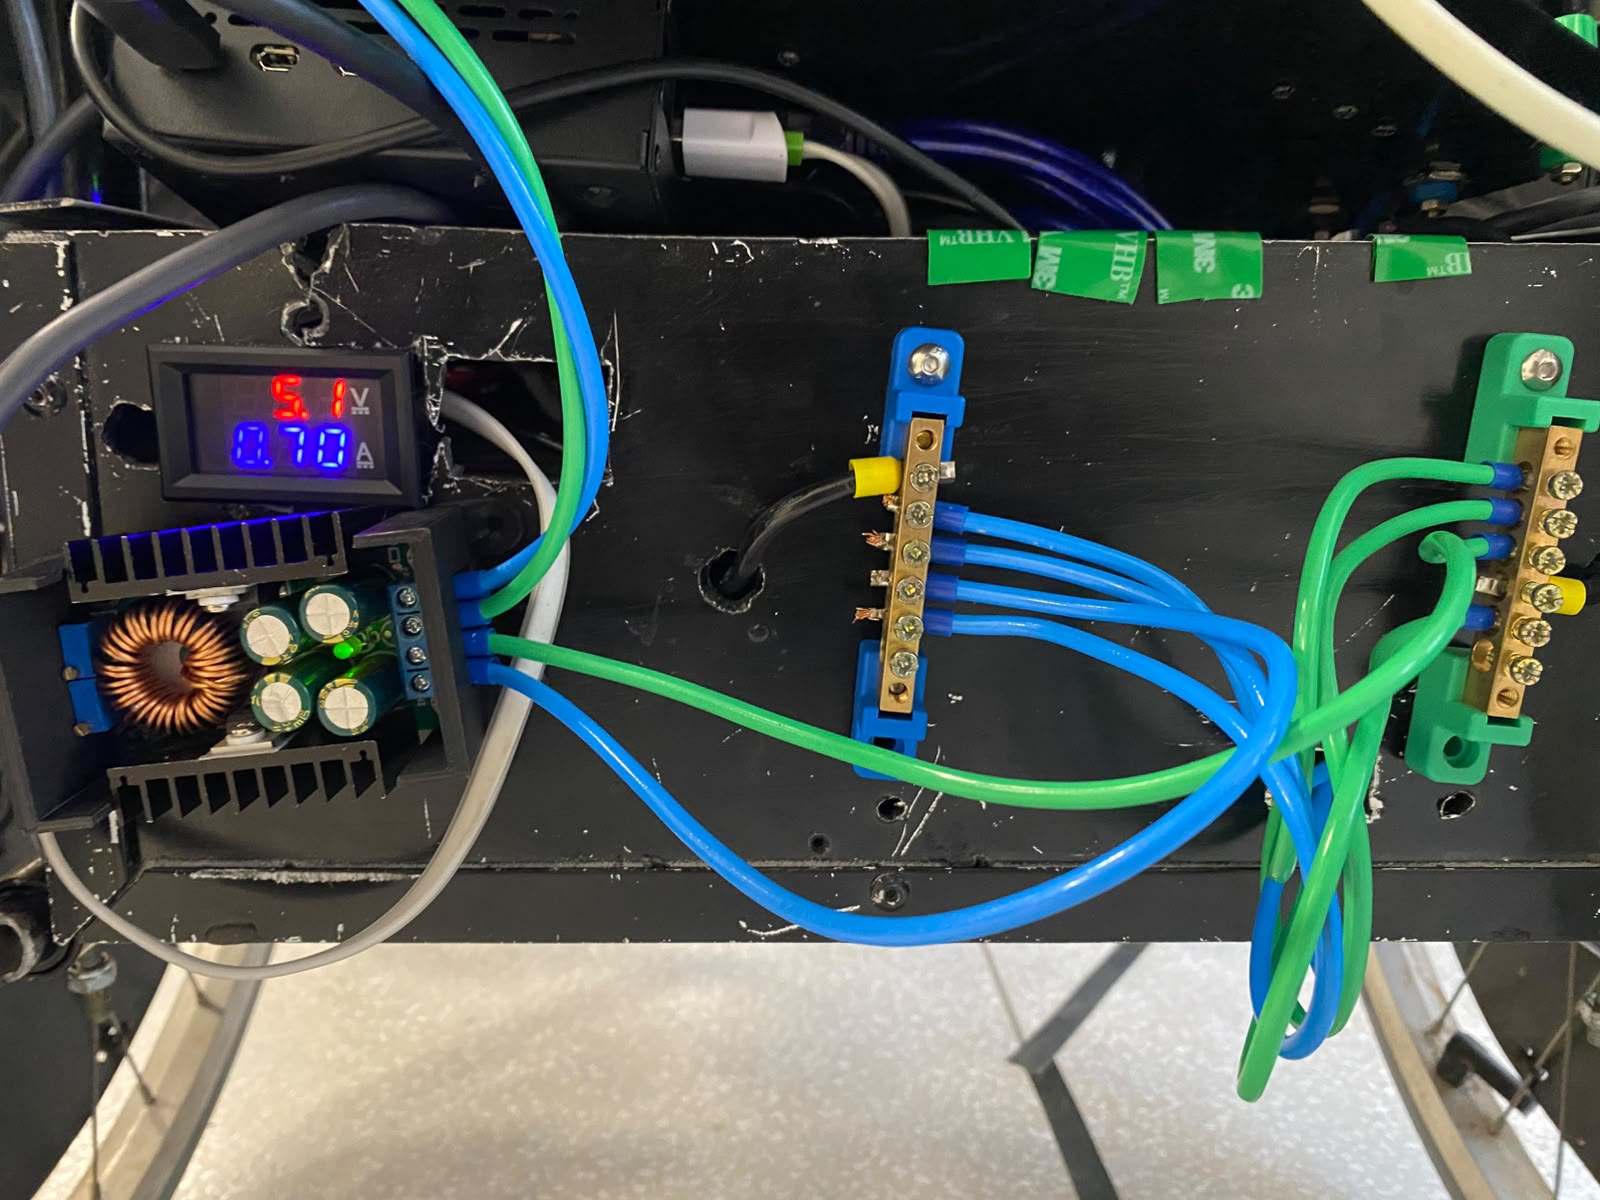
\includegraphics[width=0.48\columnwidth]{terminais_alimentacao}
\caption{À esquerda, acoplamento motor--roda e encoder no cubo. À direita,
barramento de potência: conversor \emph{buck} com instrumentação de tensão e
corrente (\SI{5.1}{\volt}, \SI{0.70}{\ampere} em repouso) e barras de distribuição.}
\label{fig:eletronica}
\end{figure}

\begin{figure}[!t]
\centering
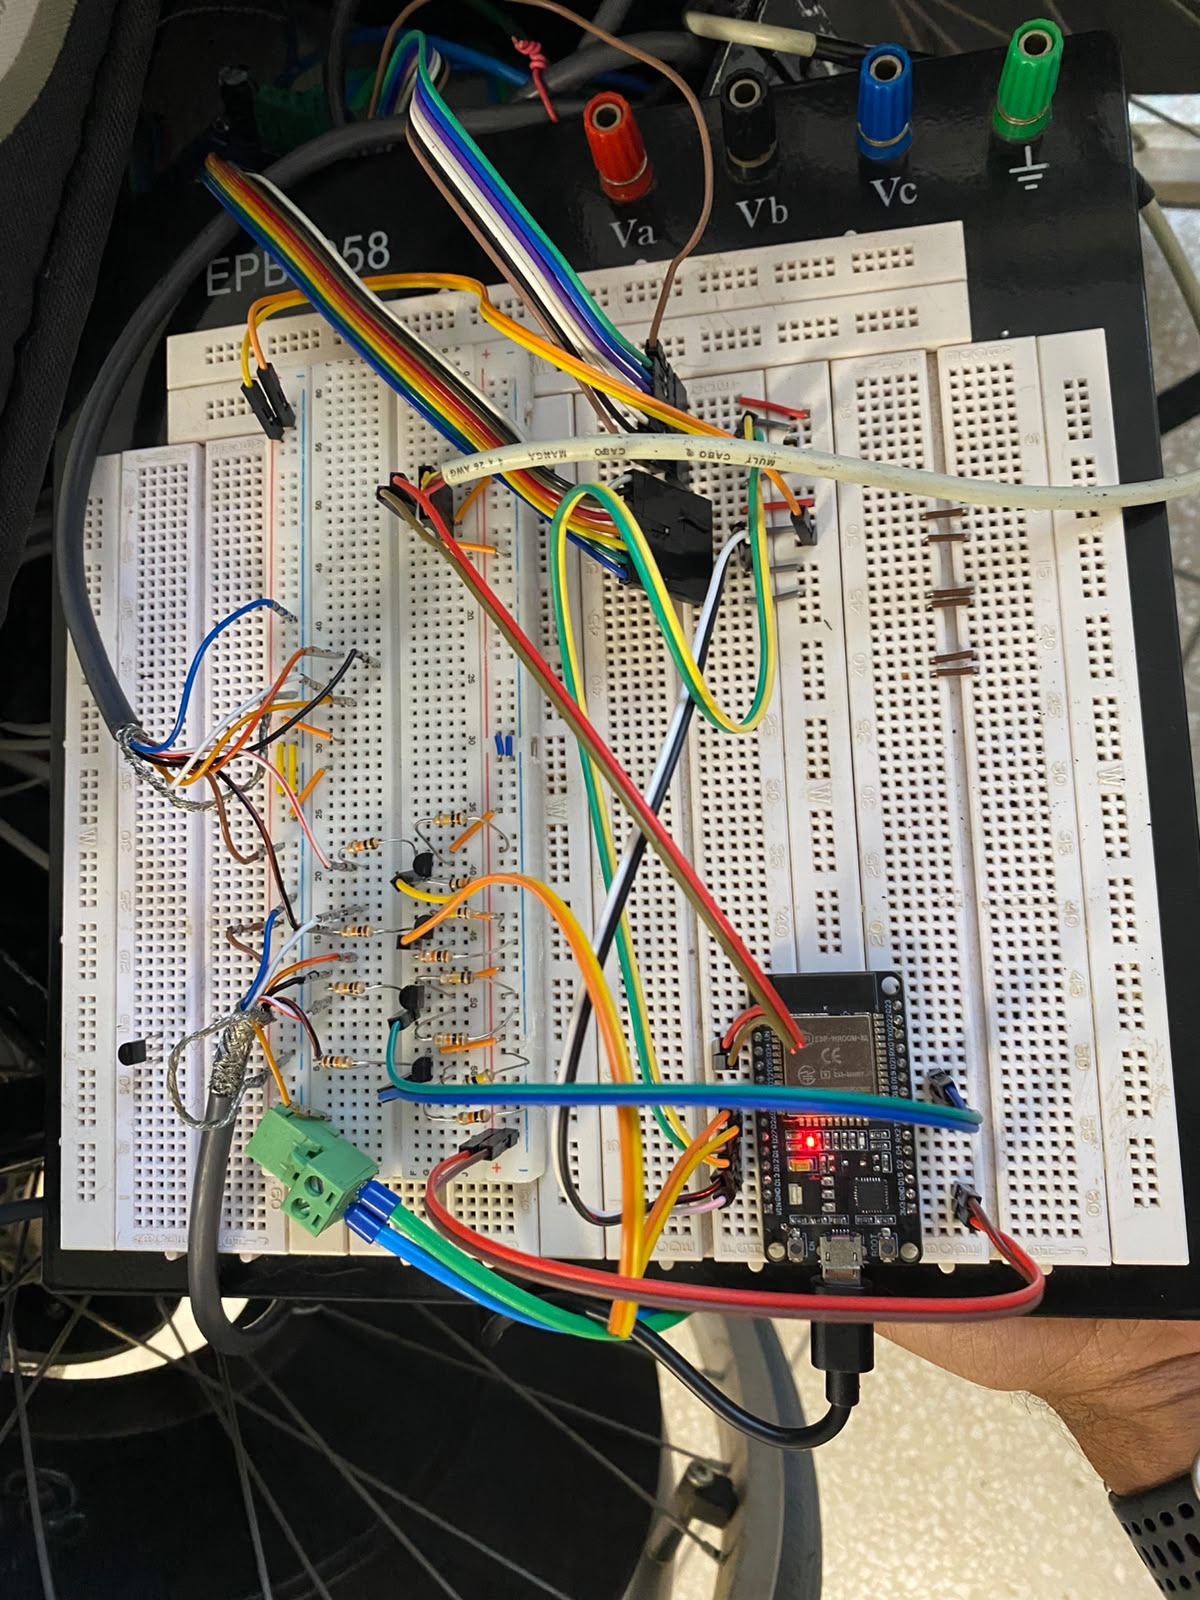
\includegraphics[width=0.72\columnwidth]{circuito_principal}
\caption{Circuito de controle montado em \emph{protoboard}: o ESP32-S3, o
condicionamento dos dois canais de encoder em quadratura e a interface com as
pontes BTS7960. O joystick analógico entra pelo ADC do próprio microcontrolador,
dispensando a placa auxiliar prevista no PC2.}
\label{fig:circuito}
\end{figure}

% =============================================================================
\section{Arquitetura}

A divisão mestre--escravo é preservada. A Fig.~\ref{fig:fluxo} resume o fluxo de
dados, agora com o caminho de \emph{retorno} de odometria fechado.

\begin{figure*}[!t]
\centering
\resizebox{0.92\textwidth}{!}{%
\begin{tikzpicture}[
  font=\footnotesize,
  every node/.style={align=center},
  blk/.style={draw, rounded corners=2pt, minimum height=10mm,
              minimum width=30mm, inner sep=4pt, fill=gray!6},
  sens/.style={draw, rounded corners=2pt, minimum height=10mm,
               minimum width=24mm, inner sep=4pt, fill=gray!14},
  arr/.style={-Latex, thick},
  lab/.style={font=\scriptsize, fill=white, inner sep=1pt}
]
\node[sens] (esp) at (0,0) {ESP32-S3 / firmware\\joystick + PID + encoders};
\node[blk]  (bridge) at (4.6,0) {\texttt{esp\_bridge}\\(ponte serial)};
\node[blk]  (shared) at (9.6,0) {\texttt{shared\_control}\\(função custo)};
\node[sens] (lidar) at (9.6,-2.0) {LiDAR\\\texttt{/scan}};
\node[blk]  (slam) at (4.6,-2.0) {\texttt{slam\_toolbox}\\+ EKF};

\draw[arr] (esp.east) -- (bridge.west)
  node[midway,above,lab] {telemetria};
\draw[arr] (bridge.east) -- (shared.west)
  node[midway,above,lab] {\texttt{/joystick\_cmd\_vel}};
\draw[arr] (lidar.north) -- (shared.south)
  node[midway,right,lab] {\texttt{/scan}};
\draw[arr] (bridge.south) -- (slam.north)
  node[midway,right,lab] {\texttt{/wheel/odom}};
\draw[arr] (shared.north) -- ++(0,0.9) -| (bridge.north)
  node[pos=0.25,above,lab] {\texttt{/cmd\_vel} (atenuado)};
\draw[arr] (bridge.west) -- ++(-1.2,0) |- (esp.north)
  node[pos=0.25,above,lab] {\texttt{drive\_cfg} + \texttt{drive\_cmd}};
\end{tikzpicture}%
}
\caption{Fluxo de dados consolidado. Em relação ao PC4, a ponte passou a integrar
a odometria de encoders e publicá-la em \texttt{/wheel/odom}, alimentando o
\texttt{slam\_toolbox} e o EKF~\cite{robotlocalization}. A iniciativa de avanço permanece sempre do
usuário; o supervisor apenas freia ou desvia.}
\label{fig:fluxo}
\end{figure*}

\subsection{Protocolo serial}

O firmware (\texttt{fw~0.9.2}) emite telemetria JSON delimitada por linha a
\SI{20}{\hertz} sobre a serial USB. Registra-se aqui uma \textbf{correção} em
relação ao PC4, que informava \num{115200}\,bps: a taxa efetiva do enlace é
\num{460800}\,bps, valor adotado também como padrão da ponte ROS\,2. As mensagens
aceitas são:

\begin{lstlisting}[basicstyle=\ttfamily\scriptsize]
{"type":"drive_cfg","armed":true,"max_duty":0.20,
 "front_lock":false}
{"type":"wheel_speed_cmd","left_rad_s":0.0,
 "right_rad_s":0.0}
{"type":"drive_cmd","left":0.0,"right":0.0}
{"type":"wheel_pid_cfg", ...}
{"type":"stop"}
\end{lstlisting}

O \texttt{drive\_cfg} permanece como portão de segurança: sua ausência por mais
que o intervalo de \emph{watchdog} desarma o estágio de potência. O
\texttt{wheel\_speed\_cmd} é a novidade da malha fechada: carrega o
\emph{setpoint} angular de cada roda, consumido pelos dois PIDs do firmware.

\subsection{Odometria de rodas}

Os encoders são lidos pelo PCNT em quadratura 4$\times$, resultando em
$N=\num{8000}$ contagens por volta de roda. Com raio $r$ e entre-eixos $L$, o
incremento de cada roda entre amostras é
\begin{equation}
\Delta D_{\{L,R\}} = \sigma \, \frac{\Delta n_{\{L,R\}}}{N} \, 2\pi r,
\end{equation}
\noindent onde $\sigma=-1$ é o sinal de encoder do \emph{hardware} atual (avanço
produz contagem negativa em ambas as rodas). A pose 2D segue a aproximação de
arco médio:
\begin{align}
\Delta s &= \frac{\Delta D_L + \Delta D_R}{2}, &
\Delta \psi &= \frac{\Delta D_R - \Delta D_L}{L},\\
x_{k+1} &= x_k + \Delta s\cos\!\Big(\psi_k+\tfrac{\Delta\psi}{2}\Big), &
\psi_{k+1} &= \psi_k + \Delta\psi .
\end{align}
Note que $\Delta s$ e $\Delta \psi$ dependem apenas de \emph{contagens}, não do
intervalo de amostragem --- propriedade que se mostrará decisiva na
Seção~\ref{sec:defeito-vel}.

\subsection{Malha de velocidade por roda}

Cada roda possui um PID que rastreia o \emph{setpoint} $\omega^\star$ recebido do
host, realimentado pela velocidade estimada dos encoders, com saturação pelo teto
de \emph{duty} vigente. A saída do controlador nunca excede o
\texttt{max\_duty} do \texttt{drive\_cfg}, de modo que o portão de segurança
permanece soberano sobre a malha de controle. O estado interno (\emph{setpoint},
velocidade medida, erro e saída) é devolvido na telemetria, permitindo sintonia e
auditoria a partir da GUI (Fig.~\ref{fig:gui-pid}) e do tópico
\texttt{/wheel/pid\_state}.

\begin{figure}[!t]
\centering
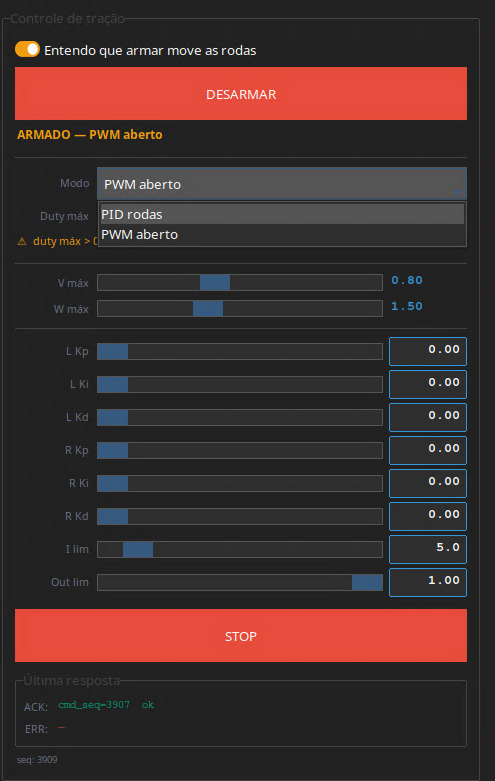
\includegraphics[width=0.60\columnwidth]{gui_ajuste_pid}
\caption{Painel de tração com o sistema armado e o seletor de modo aberto,
evidenciando as duas malhas disponíveis: \emph{PID de rodas} (realimentada por
encoder) e \emph{PWM aberto} (sem realimentação). Os ganhos de cada roda, o
limite de integrador e o limite de saída são sintonizáveis em tempo real; o botão
\textsc{stop} desarma o estágio de potência imediatamente.}
\label{fig:gui-pid}
\end{figure}

\subsection{Interface gráfica de bancada}

A interface (Fig.~\ref{fig:gui-tracao} e Fig.~\ref{fig:gui-lidar}) concentra a
operação: estado do joystick físico com inversão de eixos configurável, saída dos
motores por GPIO com indicação de sentido, encoders, seleção entre os modos
\emph{PID de rodas} e \emph{PWM aberto}, teto de \emph{duty}, ganhos do PID,
parada automática do LiDAR, IMU, odometria e ensaio de degrau. Um aviso explícito
condiciona o armar do estágio de potência ao reconhecimento de que ``armar move
as rodas''.

\begin{figure}[!t]
\centering
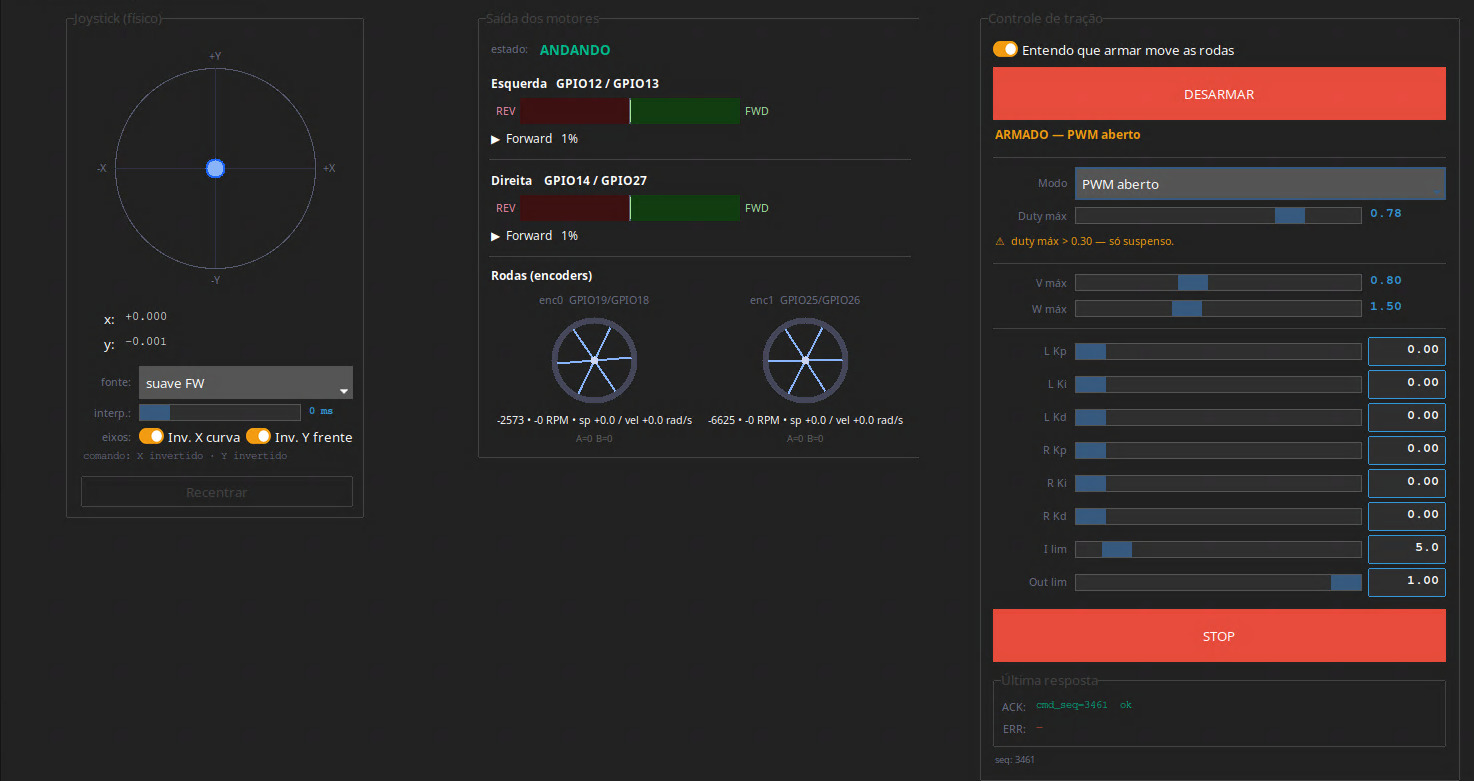
\includegraphics[width=\columnwidth]{gui_tracao}
\caption{Painéis de joystick, saída dos motores e controle de tração, com o
sistema armado em modo \emph{PWM aberto}. O aviso em âmbar sinaliza teto de
\emph{duty} acima de \num{0.30}, condição permitida apenas com a cadeira
suspensa. Observa-se a correspondência direta entre o comando e os pinos
GPIO12/13 (esquerda) e GPIO14/27 (direita).}
\label{fig:gui-tracao}
\end{figure}

\begin{figure}[!t]
\centering
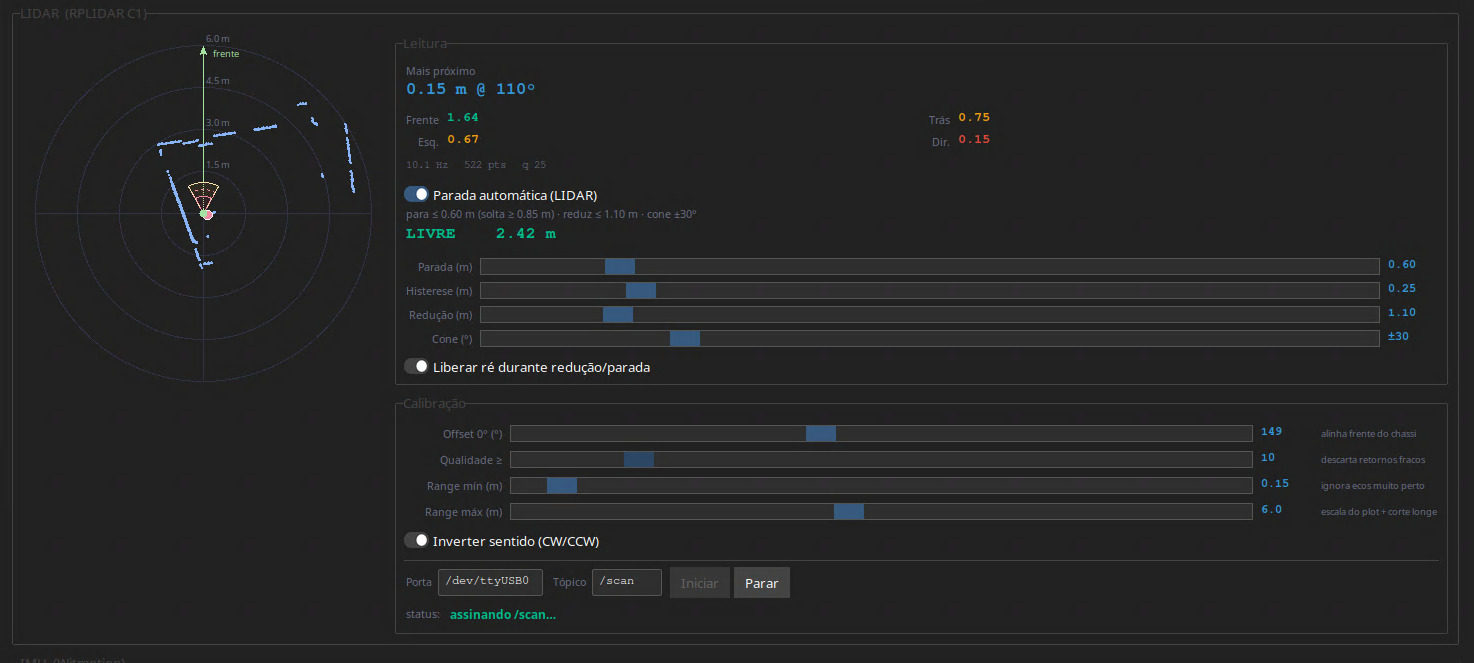
\includegraphics[width=\columnwidth]{gui_lidar}
\caption{Painel do LiDAR com parada automática habilitada. O gráfico polar mostra
a varredura a \SI{10.1}{\hertz} com \num{522} pontos válidos; o cone frontal de
$\pm 30^\circ$ está livre em \SI{2.42}{\metre}, e o retorno mais próximo
(\SI{0.15}{\metre}) é descartado como estrutura da própria cadeira.}
\label{fig:gui-lidar}
\end{figure}

% =============================================================================
\section{Resultados Experimentais}

\subsection{Experimento 1: Odometria de encoders em condução no solo}

Com o joystick recalibrado (offset de centro reajustado; leitura em repouso
$x=y=0{,}000$), a cadeira foi conduzida no solo em modo \emph{PWM aberto} com o
supervisor de LiDAR desabilitado, em área livre. O registro de odometria da GUI
foi zerado antes do ensaio e exportado ao final.

O ensaio produziu \num{2748} amostras ao longo de \SI{256}{\second}. Adotando
como critério de movimento a velocidade medida pelo firmware acima de
\SI{0.10}{\radian\per\second} em alguma das rodas, \SI{58}{\second}
(\SI{23}{\percent}) correspondem a tráfego efetivo --- ou seja, a cadeira
permaneceu parada em \SI{77}{\percent} do tempo, entre manobras. A
Tabela~\ref{tab:run} resume o ensaio, a Fig.~\ref{fig:trajetoria} mostra a
trajetória reconstruída de cada roda e a Fig.~\ref{fig:gui-odometria} registra o
painel da interface ao final da corrida.

\begin{table}[!t]
\caption{Ensaio de condução no solo (odometria de encoders)}
\label{tab:run}
\centering
\footnotesize
\renewcommand{\arraystretch}{1.2}
\begin{tabular}{@{}p{0.46\columnwidth}p{0.42\columnwidth}@{}}
\hline
\textbf{Grandeza} & \textbf{Valor} \\
\hline
Amostras / duração            & \num{2748} / \SI{256}{\second} \\
Tráfego efetivo               & \SI{58}{\second} (\SI{23}{\percent}) \\
Caminho do centro, $\sum|\Delta s|$ & \SI{9.74}{\metre} \\
Caminho por roda, $\sum|\Delta D|$ (L / R) & \SI{8.67}{\metre} / \SI{11.86}{\metre} \\
Deslocamento com sinal (L / R) & \SI{6.76}{\metre} / \SI{11.13}{\metre} \\
Extensão do trajeto           & \SI{2.26}{\metre} $\times$ \SI{2.18}{\metre} \\
Rotação total, $\sum|\Delta\psi|$ & \SI{849}{\degree} \\
Pose final $(x,y,\psi)$       & $(\num{0.240};\, \num{1.002})\,$m, \SI{490.7}{\degree} \\
Velocidade linear (pico)      & \SI{0.86}{\metre\per\second} \\
Velocidade angular (pico)     & \SI{2.29}{\radian\per\second} \\
\hline
\end{tabular}
\end{table}

\begin{figure}[!t]
\centering
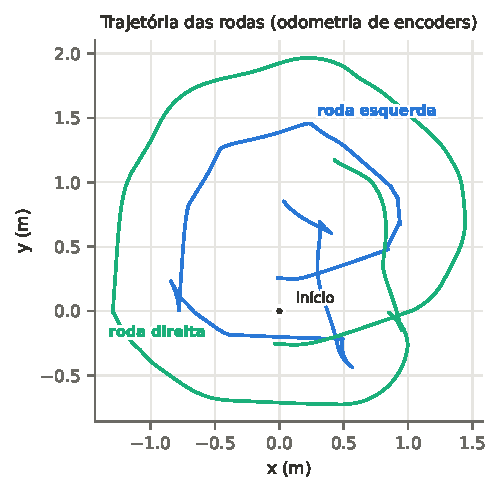
\includegraphics[width=0.86\columnwidth]{trajetoria.pdf}
\caption{Trajetória reconstruída de cada roda a partir das contagens de encoder.
O trajeto compreende duas voltas fechadas e manobras de giro no lugar; a
separação constante entre os traçados corresponde ao entre-eixos calibrado de
\SI{0.510}{\metre}. Odometria pura de rodas: sujeita a deriva acumulada.}
\label{fig:trajetoria}
\end{figure}

\begin{figure}[!t]
\centering
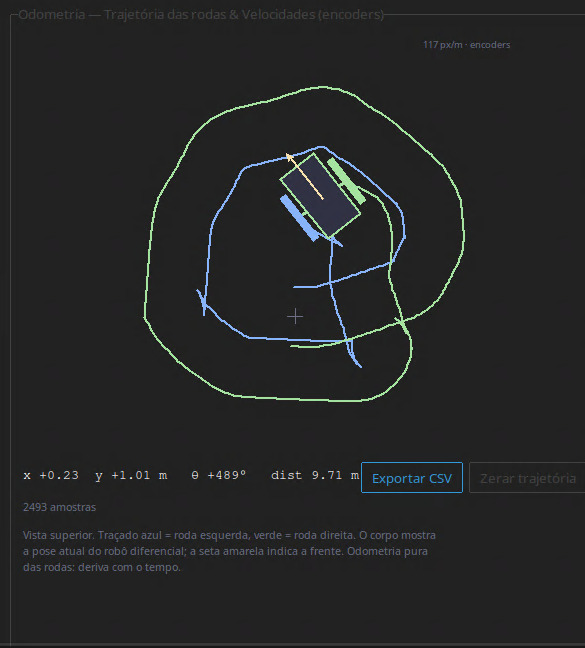
\includegraphics[width=0.66\columnwidth]{gui_odometria}
\caption{Painel de odometria da interface ao final do ensaio, com o mesmo trajeto
da Fig.~\ref{fig:trajetoria} reconstruído em tempo real. A captura foi tomada
poucos segundos antes da exportação do CSV, daí a pequena diferença nos
totais (\SI{9.71}{\metre} / \num{2493} amostras na tela contra
\SI{9.74}{\metre} / \num{2748} no arquivo). Os gráficos de velocidade da
interface foram deliberadamente omitidos desta figura pelo motivo exposto na
Seção~\ref{sec:defeito-vel}.}
\label{fig:gui-odometria}
\end{figure}

Distingue-se aqui o \emph{caminho} percorrido por cada roda ($\sum|\Delta D|$,
sempre positivo) do \emph{deslocamento com sinal} ($\sum \Delta D$, que desconta
os trechos de recuo). Só o segundo entra na cinemática diferencial. Com ele,
\begin{equation}
\Delta\psi = \frac{D_R - D_L}{L}
= \frac{\SI{11.13}{\metre}-\SI{6.76}{\metre}}{\SI{0.510}{\metre}}
= \SI{8.564}{\radian} = \SI{490.7}{\degree},
\end{equation}
\noindent exatamente o rumo final integrado (diferença nula). Cabe, porém, uma
ressalva metodológica que evita superestimar essa concordância: como $\psi$ é
integrado justamente pela soma de $(\Delta D_R - \Delta D_L)/L$, o fechamento é
uma \textbf{identidade algébrica}, não uma medição independente. Ele confirma que
a implementação da integração está aritmeticamente correta --- o que não é
trivial, dado que o sinal $\sigma$ e a ordem das rodas são fontes clássicas de
erro --- mas \emph{não} constitui evidência externa da acurácia da odometria.
Validação física exigiria fechamento de laço contra referência independente, o
que não foi possível: parar a cadeira exatamente no ponto de partida, com a
precisão necessária, mostrou-se impraticável no ensaio manual.

\subsection{Experimento 2: Velocidades e um defeito de medição}
\label{sec:defeito-vel}

As Figs.~\ref{fig:vel-rodas}, \ref{fig:vel-linear} e~\ref{fig:vel-angular}
apresentam as velocidades do mesmo ensaio. \textbf{Elas foram construídas a
partir da velocidade medida pelo firmware} (\texttt{wheel\_*\_vel\_rad\_s}), e
não das colunas homônimas calculadas pela interface. A razão é um defeito que
este ensaio expôs.

\begin{figure}[!t]
\centering
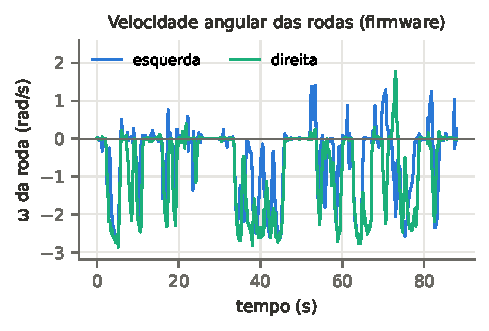
\includegraphics[width=0.94\columnwidth]{vel_rodas.pdf}
\caption{Velocidade angular de cada roda durante os \SI{58}{\second} de tráfego
efetivo. Valores negativos correspondem ao avanço ($\sigma=-1$). Os trechos em
que as rodas assumem sinais opostos são os giros no lugar visíveis na
Fig.~\ref{fig:trajetoria}.}
\label{fig:vel-rodas}
\end{figure}

\begin{figure}[!t]
\centering
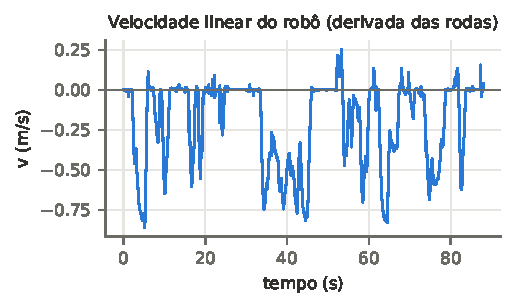
\includegraphics[width=0.94\columnwidth]{vel_linear.pdf}
\caption{Velocidade linear do robô, $v=(\omega_L+\omega_R)\,r/2$, derivada da
medição do firmware. O pico de \SI{0.86}{\metre\per\second} é compatível com a
faixa típica de cadeiras motorizadas.}
\label{fig:vel-linear}
\end{figure}

\begin{figure}[!t]
\centering
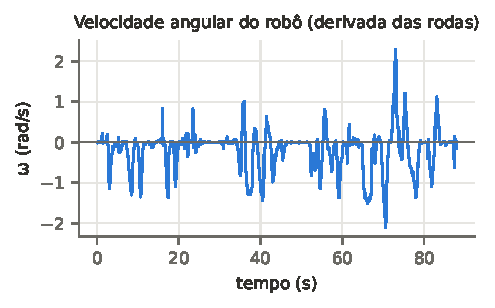
\includegraphics[width=0.94\columnwidth]{vel_angular.pdf}
\caption{Velocidade angular do robô, $\dot\psi=(\omega_R-\omega_L)\,r/L$. Os
extremos de $\pm\SI{2.3}{\radian\per\second}$ ocorrem nos giros no lugar.}
\label{fig:vel-angular}
\end{figure}

\paragraph{O defeito} A interface estimava a velocidade de cada roda como
$\Delta n/\Delta t$, adotando como $\Delta t$ o intervalo de \emph{relógio de
parede} entre as chegadas de pacotes. Como a serial entrega em rajadas, o
$\Delta t$ observado no ensaio tem mediana de \SI{98}{\milli\second} mas
\num{363} amostras (\SI{13}{\percent}) abaixo de \SI{20}{\milli\second}, com
mínimo de \SI{1}{\milli\second}. Dividir um incremento normal de contagens por
\SI{1}{\milli\second} produz velocidades absurdas. A Tabela~\ref{tab:defeito}
contrasta as duas estimativas para a roda esquerda.

\begin{table}[!t]
\caption{Velocidade da roda esquerda: firmware \emph{versus} interface}
\label{tab:defeito}
\centering
\footnotesize
\renewcommand{\arraystretch}{1.2}
\begin{tabular}{@{}lccc@{}}
\hline
\textbf{Estimador} & \textbf{p50} & \textbf{p95} & \textbf{máx} \\
\hline
Firmware (filtrado)          & \num{0.000} & \num{0.517} & \num{0.876} \\
Interface ($\Delta n/\Delta t$) & \num{0.001} & \num{1.913} & \num{14.272} \\
\hline
\multicolumn{4}{@{}l@{}}{\footnotesize Valores em \si{\metre\per\second}.
\SI{10}{\percent} das amostras da interface excedem \SI{0.6}{\metre\per\second}.}
\end{tabular}
\end{table}

O estimador da interface chega a \SI{14.27}{\metre\per\second}
(\SI{51}{\kilo\metre\per\hour}) --- dezesseis vezes o máximo físico. O defeito é
\emph{de medição, não de odometria}: pose, rumo e distância dependem apenas de
contagens (Eq.~2--3) e permanecem corretos, o que explica por que a
Fig.~\ref{fig:trajetoria} é fidedigna enquanto os gráficos de velocidade da tela
não o eram. A correção especificada é dupla: usar o carimbo temporal
\texttt{t\_ms} emitido pelo próprio firmware e impor um piso a $\Delta t$. Este é
um caso didático do tema da disciplina: \emph{a base de tempo de uma medição
embarcada não pode ser o relógio do consumidor dos dados}.

Registra-se, em contrapartida, que a coluna do firmware não exibe a mesma
patologia: isolando as amostras em que a contagem de uma roda permanece
congelada, sua velocidade estimada nunca excede \SI{0.13}{\radian\per\second}
(\SI{0.04}{\metre\per\second}), compatível com a quantização de
$1/\num{8000}$ de volta e sem picos espúrios. A estimativa embarcada, que dispõe
de base de tempo própria, dispensa portanto a filtragem adicional que a camada de
visualização exigiria.

\subsection{Experimento 3: Supervisor de segurança LiDAR}

O supervisor de bancada foi reexercitado com o LiDAR RPLIDAR~C1~\cite{slamtec} publicando
\texttt{/scan} a \SI{10.1}{\hertz} com \num{522} pontos por varredura
(Fig.~\ref{fig:gui-lidar}). A lógica de zonas confirma-se conforme projetada e
sintetizada na Tabela~\ref{tab:zonas}: teto nominal com frente livre, redução
proporcional na zona amarela e teto nulo na zona vermelha, com histerese de
\SI{0.25}{\metre} para evitar oscilação no limiar. Retornos abaixo de
\SI{0.15}{\metre} são descartados como estrutura da própria cadeira.

A folga frontal, contudo, é medida por um \emph{cone angular que nasce no
sensor}. Essa construção pressupõe tacitamente que o LiDAR esteja sobre o eixo
longitudinal da cadeira. Ele não está --- e a Seção~\ref{sec:corredor} mostra que
essa premissa, e não a lógica de zonas, é a origem de uma falha de segurança.

\begin{table}[!t]
\caption{Resposta da parada automática à folga frontal}
\label{tab:zonas}
\centering
\footnotesize
\renewcommand{\arraystretch}{1.2}
\begin{tabular}{@{}p{0.24\columnwidth}p{0.20\columnwidth}p{0.42\columnwidth}@{}}
\hline
\textbf{Folga frontal} & \textbf{Zona} & \textbf{Teto de \emph{duty}} \\
\hline
$\le \SI{0.60}{\metre}$      & vermelha & $0$ (parada); solta em \SI{0.85}{\metre} \\
\SIrange{0.60}{1.10}{\metre} & amarela  & reduzido linearmente com a folga \\
$> \SI{1.10}{\metre}$        & livre    & nominal \\
$< \SI{0.15}{\metre}$        & ignorada & descartada (estrutura) \\
\hline
\end{tabular}
\end{table}

\subsection{Experimento 4: Um defeito geométrico no supervisor --- do cone ao corredor}
\label{sec:corredor}

Em ensaios de condução com o supervisor armado, observou-se repetidamente que a
cadeira \textbf{ignorava obstáculos levemente deslocados à direita e os
atropelava}, embora parasse corretamente diante de obstáculos centrados. O mesmo
supervisor exibia um segundo sintoma, aparentemente não relacionado: com
$K_{\text{assist}}>0$, ele \emph{parava} sem nunca \emph{desviar}. Ambos têm uma
única causa, e ela não está na lógica de zonas.

\paragraph{A premissa oculta} Medir a folga por um cone angular só é válido se o
vértice do cone coincidir com o eixo longitudinal do veículo. Mediu-se a
montagem real: o LiDAR está a \SI{0.667}{\metre} à frente do eixo traseiro,
\SI{0.336}{\metre} \textbf{à esquerda} do eixo longitudinal (\SI{0.05}{\metre}
para fora da roda esquerda) e a \SI{0.15}{\metre} do solo. Com o vértice
deslocado, o cone varre uma faixa igualmente deslocada. A
Tabela~\ref{tab:cobertura} quantifica a fração da largura da cadeira
(\SI{0.61}{\metre}) efetivamente monitorada.

\begin{table}[!t]
\caption{Fração da largura da cadeira coberta pelo cone, por folga frontal}
\label{tab:cobertura}
\centering
\footnotesize
\renewcommand{\arraystretch}{1.2}
\begin{tabular}{@{}p{0.16\columnwidth}p{0.34\columnwidth}p{0.34\columnwidth}@{}}
\hline
\textbf{Folga} & \textbf{Cone $\pm30^\circ$ (GUI)} & \textbf{Cone $\pm20^\circ$ (ROS\,2)} \\
\hline
\SI{0.30}{\metre} & \SI{23}{\percent} & \SI{13}{\percent} \\
\SI{0.60}{\metre} & \SI{52}{\percent} & \SI{31}{\percent} \\
\SI{1.00}{\metre} & \SI{90}{\percent} & \SI{55}{\percent} \\
\SI{1.50}{\metre} & \SI{100}{\percent} & \SI{84}{\percent} \\
\hline
\multicolumn{3}{@{}p{0.86\columnwidth}@{}}{\footnotesize A parcela não coberta é
\emph{sempre} a metade direita. Na distância de parada (\SI{0.60}{\metre}), o
cone de $\pm30^\circ$ enxerga apenas $Y>\SI{-0.01}{\metre}$: todo o lado direito
da cadeira é cego exatamente onde a parada precisa agir.}
\end{tabular}
\end{table}

O resultado é contraintuitivo mas rigoroso: a cobertura \emph{piora} à medida que
o obstáculo se aproxima, porque o cone estreita enquanto o desvio lateral do
vértice permanece constante. Isso explica os dois sintomas de uma só vez. Um
obstáculo à direita nunca entra no cone e é atropelado; e um obstáculo
descentralizado que \emph{acaba} entrando só o faz muito perto, fazendo a folga
saltar de um valor acima da zona amarela diretamente para dentro da zona
vermelha --- sem trecho intermediário em que o desvio pudesse arquear a
trajetória. Não existe, portanto, um valor ``melhor'' de \texttt{front\_offset}:
\textbf{nenhum ângulo único representa ``a frente'' quando o sensor está fora do
eixo}.

\paragraph{A correção} A função custo que escolhe a direção de desvio é
aparentada ao \emph{Vector Field Histogram}~\cite{borenstein1991}, que também
pontua direções candidatas pela folga. O VFH, porém, raciocina sobre a
\emph{planta} do robô, não sobre um cone ancorado no sensor --- distinção que
aqui se mostrou decisiva. Substituiu-se, pois, o cone pelo teste do
\emph{corredor físico} que a cadeira ocupará. Cada retorno $(a,r)$ é projetado no \texttt{base\_link},
\begin{align}
X &= x_L + r\cos(a + \theta_L), &
Y &= y_L + r\sin(a + \theta_L),
\end{align}
\noindent e classificado como obstáculo se $X > X_f$ e $|Y| \le W/2$, com folga
$X - X_f$; aqui $(x_L,y_L,\theta_L)$ é a pose do sensor, $X_f$ a frente do
chassi e $W$ a largura. Para avaliar um desvio candidato $\delta$, giram-se os
pontos por $-\delta$ em torno do eixo traseiro, que é o centro instantâneo de
rotação do acionamento diferencial. A Fig.~\ref{fig:corredor} contrasta as duas
geometrias.

\begin{figure}[!t]
\centering
\begin{tikzpicture}[scale=2.05, font=\scriptsize]
  \definecolor{blind}{RGB}{200,60,60}
  \definecolor{corr}{RGB}{70,130,180}
  % --- corredor da cadeira (o que ela de fato ocupa) ---
  \fill[corr, opacity=0.16] (0.667,-0.305) rectangle (1.75,0.305);
  % --- cone +-30 deg com vertice no sensor (0.667, 0.336) ---
  \fill[blind, opacity=0.10] (0.667,0.336) -- (1.7495,0.9610) -- (1.7495,-0.2890) -- cycle;
  \draw[blind, thick, dashed] (0.667,0.336) -- (1.7495, 0.9610);
  \draw[blind, thick, dashed] (0.667,0.336) -- (1.7495,-0.2890);
  % --- zona cega: corredor abaixo do raio inferior do cone ---
  \fill[blind, opacity=0.40]
    (0.667,-0.305) -- (1.7495,-0.305) -- (1.7495,-0.2890)
    -- (0.7207,0.305) -- (0.667,0.305) -- cycle;
  % --- chassi ---
  \draw[thick, fill=gray!8] (-0.30,-0.305) rectangle (0.667,0.305);
  \draw[dashed, gray] (-0.36,0) -- (1.80,0);
  \draw[fill=black] (0,0) circle (0.017);
  \node[below left=0pt] at (0,0) {\texttt{base\_link}};
  % rodas motorizadas
  \draw[line width=1.8pt] (-0.05,-0.305) -- (0.09,-0.305);
  \draw[line width=1.8pt] (-0.05, 0.305) -- (0.09, 0.305);
  % --- sensor ---
  \draw[fill=blind] (0.667,0.336) circle (0.020);
  \node[blind, above=1pt] at (0.667,0.336) {LiDAR};
  % --- rotulos ---
  \node[blind] at (1.14,-0.19) {\textbf{cego}};
  \node[corr]  at (1.42,0.15) {\textbf{corredor}};
  % --- cotas ---
  \draw[<->, gray] (1.80,-0.305) -- (1.80,0.305)
    node[midway, right, black] {$W$};
  \draw[<->, gray] (0,-0.40) -- (0.667,-0.40)
    node[midway, below, black] {$X_f=\SI{0.667}{\metre}$};
  \draw[<->, gray] (0.60,0) -- (0.60,0.336)
    node[midway, left, black] {$y_L$};
\end{tikzpicture}
\caption{Vista superior. O cone (tracejado) nasce no LiDAR, deslocado
\SI{0.336}{\metre} à esquerda do eixo, e por isso deixa descoberta uma cunha à
direita (hachurada) que cresce quanto \emph{mais perto} está o obstáculo. O
corredor (azul) é definido no \texttt{base\_link} e coincide com a área que a
cadeira de fato ocupará. A estrutura do chassi, atrás de $X_f$, é excluída por
construção.}
\label{fig:corredor}
\end{figure}

\paragraph{Calibração} A pose do sensor foi medida, não arbitrada. O avanço
$x_L$ resultou de três métodos independentes --- trilateração a partir dos
centros das rodas (\SI{0.656}{\metre}) e distância perpendicular a duas paredes
(\SI{0.669}{\metre} e \SI{0.665}{\metre}) --- com espalhamento de
\SI{1.3}{\centi\metre}; adotou-se \SI{0.667}{\metre}. O desvio lateral $y_L$ veio
da trilateração (\SI{0.336}{\metre}), grandeza que o método da parede não observa.
O \emph{yaw} $\theta_L$, que a fita não mede bem, obteve-se ajustando uma reta por
mínimos quadrados totais aos pontos de uma parede plana, com a cadeira alinhada
perpendicularmente a ela (distâncias iguais das duas rodas traseiras): a
orientação de uma reta é invariante à translação, de modo que $\theta_L$ sai
sem depender da posição do sensor. Duas paredes, a \SI{2.75}{\metre} e a
\SI{2.18}{\metre}, forneceram $\theta_L=\SI{-155.46}{\degree}$ e
$\theta_L=\SI{-154.97}{\degree}$ (planicidade RMS de \SI{5.8}{\milli\metre} e
\SI{5.5}{\milli\metre}); adotou-se \SI{-155.22}{\degree}, com dispersão entre as
duas paredes de \SI{0.49}{\degree}.

\paragraph{Validação} Com a cadeira perpendicular a uma parede a
\SI{2.18}{\metre} do eixo traseiro, o corredor deve reportar
$\SI{2.18}{\metre}-X_f=\SI{1.513}{\metre}$. O supervisor reportou
\SI{1.509}{\metre}: erro de \SI{4}{\milli\metre} contra referência física
independente. A cobertura tornou-se simétrica --- na mesma varredura, \num{21}
pontos na metade direita do corredor contra \num{23} na esquerda, onde antes a
direita era essencialmente vazia. Dois efeitos colaterais benéficos: os retornos
da própria estrutura (a \SI{0.07}{\metre} e \SI{0.49}{\metre}) caem atrás de
$X_f$ e são descartados sem necessidade do limiar \texttt{min\_obstacle\_range};
e a projeção vetorizada, executada uma vez por varredura, reduziu o custo do nó
de \SI{17.7}{\percent} para \SI{8.3}{\percent} de CPU \emph{fazendo mais
trabalho} (\num{19} candidatos $\times$ \num{564} pontos), preservando o laço de
controle a \SI{20}{\hertz}.

\paragraph{Um segundo defeito: ângulo somado como taxa} Corrigida a geometria e
exercitado o desvio com motor, a cadeira passou a executar giros de até
$\approx 180^\circ$ em vez de contornar o obstáculo. A causa é uma inconsistência
dimensional: a função custo devolve $\delta^\star$, um \emph{offset de rumo}
(rad), que era somado diretamente à velocidade angular do usuário,
$\omega_{\text{out}} = \omega_{\text{usr}} + K_{\text{assist}}\,\delta^\star$.
Uma grandeza de ângulo aplicada a cada ciclo de controle torna-se uma
\emph{taxa sustentada}: com $K_{\text{assist}}=0{,}8$ e
$\delta^\star=45^\circ$, resultam \SI{0.63}{\radian\per\second} mantidos enquanto
o obstáculo permanecer na zona amarela --- a cadeira pirueta até a frente abrir.
A correção reconhece que esterçar é \emph{curvatura vezes velocidade}:
\begin{equation}
\omega_{\text{out}} = \omega_{\text{usr}} +
\operatorname{sat}\!\big(K_{\text{assist}}\,\delta^\star\, v_{\text{out}}\big),
\end{equation}
\noindent escalando pelo avanço efetivo $v_{\text{out}}$ e saturando a taxa
injetada. Assim a cadeira \emph{arqueia} em vez de girar no lugar, o desvio
desaparece junto com o avanço --- pirueta parada torna-se impossível --- e o
supervisor nunca domina o comando do usuário. Este defeito é instrutivo por ser
invisível à análise dimensional informal: ambos os termos ``parecem'' rotação.

Registra-se, para não superestimar o resultado, que esta validação é
\emph{geométrica}: ela prova que o supervisor mede a folga correta e enxerga os
dois lados. O comportamento sob movimento --- em particular a distância de
frenagem real a partir do teto de \emph{duty} elevado, e a eficácia do desvio
corrigido --- ainda não foi caracterizado quantitativamente.

\subsection{Experimento 5: Bloqueio direcional --- implementado, não validado}
\label{sec:frontlock}

O PC4 apontou como limitação que a parada por teto de \emph{duty} inibe também a
ré nas proximidades do obstáculo, e propôs como trabalho futuro um
\emph{bloqueio direcional}: travar apenas o avanço, preservando a manobra de
recuo. Essa funcionalidade foi implementada nesta etapa em duas camadas: um sinal
\texttt{front\_lock} acrescentado ao \texttt{drive\_cfg}, e uma trava no
\emph{driver} de PWM que força os pinos de avanço a nível baixo.

\textbf{A funcionalidade não é reportada como validada.} Uma revisão de código
identificou uma inconsistência de convenção de sinal entre as duas camadas: o
host trata comando positivo como avanço para \emph{ambas} as rodas, enquanto a
trava do \emph{driver} bloqueia comando positivo na roda esquerda e comando
\emph{negativo} na roda direita. Sob a convenção do host, o efeito líquido com a
trava ativa seria (i)~não bloquear o avanço da roda direita se um comando chegar
por um caminho que contorne a camada de interface, e (ii)~anular a ré dessa mesma
roda, fazendo a cadeira pivotar em vez de recuar em linha reta --- exatamente o
oposto da intenção de projeto. O firmware com essa alteração \textbf{não foi
gravado no microcontrolador}, e os ensaios deste relatório foram conduzidos com a
versão \texttt{0.9.2}, que não contém a trava.

A resolução requer um ensaio de bancada com rodas suspensas para determinar
empiricamente qual sinal de comando produz rotação para a frente na roda direita,
que é montada espelhada, seguido da correção da camada divergente. Reporta-se o
defeito em vez de omiti-lo porque se trata de código de segurança: uma trava que
falha em bloquear o avanço é pior que a ausência de trava, pois induz confiança
indevida.

\subsection{Experimento 6: Robustez operacional e integridade do enlace}

Três modos de falha foram observados e tratados ao longo da integração:

\begin{itemize}
\item \textbf{Contenção da porta serial.} O nó \texttt{esp\_bridge} e a interface
gráfica disputam a mesma porta. Como o \texttt{pyserial} não estabelece bloqueio
exclusivo em Linux, dois leitores coexistem e cada um recebe fragmentos do fluxo,
produzindo falhas de \emph{parsing} silenciosas. A operação exige que apenas um
consumidor detenha o enlace por vez.

\item \textbf{Re-enumeração USB e estado inválido do microcontrolador.} Ciclos
repetidos de abertura e fechamento da porta pulsam, via CP2102, as linhas de
\emph{reset} e \emph{boot} do ESP32-S3. Observou-se a placa entrar em estado no
qual emitia apenas ruído em qualquer taxa --- uma varredura de \num{12} taxas
padrão não produziu quadro válido algum. Um replug do cabo USB não recuperou o
sistema, pois o microcontrolador é alimentado à parte; apenas o \emph{reset}
físico da placa restaurou a telemetria. Confirma-se, assim, a recomendação do PC4
de alimentar o barramento por \emph{hub} com fonte própria.

\item \textbf{Queda da ponte.} O \texttt{esp\_bridge} passou a religar
automaticamente em falha de serial, e a inicialização \emph{headless} por
\texttt{systemd} com \emph{symlinks} \texttt{udev} elimina a dependência da ordem
de enumeração.
\end{itemize}

Os \emph{failsafes} de temporização, já validados no PC4, permanecem: a expiração
do \texttt{drive\_cfg} desarma o estágio de potência e a expiração do
\texttt{wheel\_speed\_cmd} ou do \texttt{drive\_cmd} interrompe o movimento sem
retorno silencioso ao modo manual.

% =============================================================================
\section{Conclusões}

O sistema atingiu o objetivo central: uma cadeira de rodas motorizada com laço de
velocidade fechado por roda, odometria de encoders exercitada em condução no solo
e um supervisor de segurança baseado em LiDAR que pode \emph{frear}, mas nunca
\emph{acelerar}. O resultado mais relevante desta etapa, contudo, não foi
aditivo: exercitar o supervisor com motor revelou que sua noção de folga frontal
era geometricamente inválida para a montagem real do sensor, cegando a metade
direita da cadeira. Uma proteção que falha silenciosamente em parte do seu campo
é pior que a ausência de proteção, pois induz confiança indevida --- e este
princípio orientou tanto a investigação quanto a redação deste relatório. A
Tabela~\ref{tab:status} resume a situação final.

\begin{table}[!t]
\caption{Situação dos subsistemas ao final do projeto}
\label{tab:status}
\centering
\footnotesize
\renewcommand{\arraystretch}{1.2}
\begin{tabular}{@{}p{0.26\columnwidth}p{0.22\columnwidth}p{0.40\columnwidth}@{}}
\hline
\textbf{Subsistema} & \textbf{Status} & \textbf{Observação} \\
\hline
Odometria de encoders     & Operacional  & Ensaio no solo: \SI{9.74}{\metre}; consistência interna verificada, sem referência externa. \\
PID de velocidade         & Operacional  & Estado publicado em telemetria. \\
LiDAR / \texttt{/scan}    & Operacional  & \SI{10.1}{\hertz}, \num{522} pontos/varredura. \\
Geometria do supervisor   & \textbf{Corrigida} & Cone $\to$ corredor; pose do sensor calibrada (Seç.~\ref{sec:corredor}). \\
Parada automática         & Validada (geom.) & Folga aferida contra parede: erro de \SI{4}{\milli\metre}. Frenagem sob movimento não caracterizada. \\
Desvio autônomo           & \textbf{Corrigido} & Ângulo somado como taxa; agora escalado por $v_{\text{out}}$ e saturado. \\
\emph{Failsafes}          & Validados    & \emph{Watchdogs} de \texttt{drive\_cfg} e comandos. \\
Interface de bancada      & Operacional  & Painéis, ensaio de degrau, exportação CSV. \\
Autostart \emph{headless} & Operacional  & \texttt{systemd} + \texttt{udev}. \\
Medição de velocidade (GUI) & \textbf{Diagnosticada} & Defeito medido; correção especificada, não aplicada. \\
Bloqueio direcional       & \textbf{Não validado} & Defeito de sinal conhecido; não gravado. \\
Energia USB (Pi 5)        & Mitigada     & \emph{Hub} alimentado recomendado. \\
\hline
\end{tabular}
\end{table}

Como limitações honestas, registram-se: (i)~o bloqueio direcional permanece com
defeito conhecido e não gravado (Seção~\ref{sec:frontlock}); (ii)~a validação do
corredor é geométrica --- a distância de frenagem sob teto de \emph{duty} elevado
e a eficácia do desvio corrigido não foram caracterizadas quantitativamente em
movimento; (iii)~o fechamento apresentado no Experimento~1 é uma identidade
algébrica, de modo que a acurácia da odometria carece de referência externa;
(iv)~a odometria é puramente de rodas e acumula deriva, sendo a fusão com IMU e
SLAM o caminho natural; e (v)~há divergência de calibração entre a interface
(aro \SI{24}{\inch}, entre-eixos \SI{0.510}{\metre}) e a ponte ROS\,2
($r=\SI{0.293}{\metre}$, $L=\SI{0.522}{\metre}$), que deve ser unificada a partir
de um ensaio de calibração único. Observa-se que essa divergência é da mesma
natureza do defeito da Seção~\ref{sec:corredor}: parâmetros geométricos
\emph{assumidos} em vez de \emph{medidos}.

Os próximos passos são:
\begin{enumerate}
\item determinar em bancada, com rodas suspensas, a convenção de sinal da roda
direita e corrigir o bloqueio direcional, revalidando avanço \emph{e} ré;
\item caracterizar a distância de frenagem em função do teto de \emph{duty} e da
velocidade, aferindo se a zona de \SI{0.60}{\metre} é suficiente --- o supervisor
corta o comando, mas não freia ativamente;
\item unificar a calibração de aro e entre-eixos entre a GUI e a ponte ROS\,2,
adotando o mesmo protocolo de medição da Seção~\ref{sec:corredor};
\item aplicar a correção da base de tempo da velocidade na interface
(carimbo \texttt{t\_ms} do firmware e piso de $\Delta t$);
\item validar o desvio corrigido em condução, com obstáculos deslocados
lateralmente para os \emph{dois} lados do corredor;
\item obter referência externa de pose (fechamento de laço marcado no piso) para
quantificar a deriva da odometria;
\item alimentar o barramento USB por \emph{hub} com fonte própria.
\end{enumerate}

% =============================================================================
\begin{thebibliography}{99}

\bibitem{fehr2000}
L.~Fehr, W.~E. Langbein e S.~B. Skaar, ``Adequacy of power wheelchair
control interfaces for persons with severe disabilities: A clinical
survey,'' \emph{Journal of Rehabilitation Research and Development},
vol.~37, no.~3, pp.~353--360, 2000.

\bibitem{borenstein1991}
J.~Borenstein e Y.~Koren, ``The Vector Field Histogram --- Fast Obstacle
Avoidance for Mobile Robots,'' \emph{IEEE Transactions on Robotics and
Automation}, vol.~7, no.~3, pp.~278--288, 1991.

\bibitem{ogata2010}
K.~Ogata, \emph{Engenharia de Controle Moderno}, 5\textsuperscript{a}~ed.
São Paulo, SP: Pearson Prentice Hall, 2010.

\bibitem{branco2018}
M.~D.~C.~C. Branco, ``Desenvolvimento de um protótipo de cadeira de rodas
motorizada controlada por movimentos oculares,'' Trabalho de Conclusão
de Curso, UFRN, Natal, 2018.

\bibitem{ros2docs}
Open Robotics, ``Robot Operating System 2 (ROS\,2) Jazzy Jalisco
Documentation,'' 2024. Disponível em:
\url{https://docs.ros.org/en/jazzy/}.

\bibitem{robotlocalization}
T.~Moore e D.~Stouch, ``A Generalized Extended Kalman Filter
Implementation for the Robot Operating System,'' em \emph{Proceedings of
the 13th International Conference on Intelligent Autonomous Systems},
Springer, 2014.

\bibitem{slamtec}
Slamtec, ``RPLIDAR Low Cost 360 Degree Laser Range Scanner Datasheet,''
2020.

\end{thebibliography}

\end{document}
